% !TeX spellcheck = de_DE
% !TeX root = kristallographie_skript.tex

\subsubsection{Punktgruppen}

\begin{definition}[Punktgruppen]
Sei $G\leq\Isom(\IR^n)$ eine Gruppe von Bewegungen. Wenn es ein $x\in\IR^n$ gibt, das ein Fixpunkt von $G$ ist, d.h.
\[\forall g\in G: g(x)=x\]
dann nennt man $G$ eine \udot{Punktgruppe}. Ist zusätzlich auch $G\leq\Aut(\Lambda)$ erfüllt für einen Kristall $\Lambda\subseteq\IR^n$, dann nennt man $G$ eine \udot{kristallographische Punktgruppe}.
\end{definition}

\begin{lemma}[Punktgruppen vs. endliche Untergruppen]
Sei $G\leq\Isom(\IR^n)$ eine Gruppe von Bewegungen.
\begin{enumerate}
\item Ist $G$ endlich, dann ist $G$ eine Punktgruppe.
\item Ist $G$ kristallographisch, dann ist $G$ endlich.
\end{enumerate}
\end{lemma}
\begin{proof}
a. Wir haben das eigentlich schon einmal bewiesen: Wenn $x$ ein beliebiger Punkt und $G$ endlich ist, dann ist
\[\frac{1}{\abs{G}} \sum_{g\in G} g(x)\]
ein Fixpunkt von ganz $G$.

\medbreak
b. Wir wählen uns ein Koordinatensystem so, dass der Nullpunkt ein Fixpunkt wird. Starre Bewegungen, die den Nullpunkt fixieren, sind orthogonale Abbildungen.

Wir wählen drei Punkte $a_1,a_2,a_3\in\Lambda$ im Kristall in drei unabhängige Richtungen von $0$ aus. Sei $r:=\max\Set{\norm{a_1},\norm{a_2},\norm{a_3}}$. Aufgrund der Mindestabstand-Bedingung für Kristalle ist
\[X:=\Set{a\in\Lambda | \norm{a}\leq r}\]
endlich. Ist $g\in\Aut(\Lambda)$ und $g(0)=0$, so sind die drei Punkte $g(a_1),g(a_2),g(a_3)$ wieder aus $X$. Weil $a_1,a_2,a_3$ linear unabhängig sind und $g$ als orthogonale Abbildung linear ist, ist $g$ eindeutig festgelegt durch diese drei Bildpunkte. Es gibt also maximal $\abs{X}^3$ viele Elemente von $G$.
\end{proof}

\begin{remark}
Nicht jede endliche Punktgruppe ist auch eine kristallographische Gruppe. Wir werden gleich z.B. sehen, dass die Ikosaedergruppe zwar endlich, aber nicht kristallographisch ist.
\end{remark}

\subsubsection{Kristallklassen und Kristallsysteme}

\begin{remark}
Wir wissen, dass es nur eine sehr begrenzte Anzahl von (Konjugationsklassen von) endlichen Untergruppen von $O(\IR^3)$ gibt und wir haben eine Liste, die wir gut verstehen. In der Tat gibt es in jeder Dimension immer nur endlich viele endliche Untergruppen von $O(\IR^n)$.

Es bietet sich daher an, Kristalle danach zu klassifizieren, welche Punktgruppen sie haben. Naiv könnte man einfach die Punktgruppe $\Aut(\Lambda)_0$ betrachten, d.h. die Untergruppe aller derjenigen Symmetrien $g\in\Aut(\Lambda)$, die $g(0)=0$ erfüllen. Das Problem dabei ist, dass es außer der Identität überhaupt keine Symmetrien im Kristall geben muss, die den Nullpunkt festlassen. Der Nullpunkt könnte schlecht gewählt sein relativ zum Kristall, sodass er von keiner der möglichen, von $\id$ verschiedenen Drehung, keiner Spiegelung oder Drehinversion festgelassen wird (was ja die einzigen Bewegungen sind, die überhaupt Fixpunkte haben).

Und selbst wenn das nicht der Fall ist, könnte es sein, dass gar keine von $\id$ verschiedenen Drehungen, Spiegelungen oder Drehinversionen in $\Aut(\Lambda)$ existieren; jede Symmetrie könnte eine Translation, eine Schraubung oder Gleitspiegelung sein. Dann hätten wir keine Information gewonnen und würden viele sehr verschieden aussehende Kristalle in eine gemeinsame Kategorie \enquote{triviale Punktgruppe} einordnen.

Wenn wir das nicht wollen (und das wollen wir nicht), müssen wir uns überlegen, wie wir Symmetrien erfassen, die einen Translationsanteil $\neq 0$ haben, aber nicht gleich einer Translation sind, und wir den translationsfreien Anteil zweier solcher Symmetrien unterscheiden. Es stellt sich heraus, dass es eine andere, vom Kristall bestimmte Punktgruppe gibt, die das für uns tut.
\end{remark}

\begin{remark}
Wir erinnern uns, dass jede Bewegung $g:\IR^n\to\IR^n$ sich nach Wahl eines Nullpunkts schreiben lässt als Anwendung einer orthogonalen Bewegung $Q$ gefolgt von einer Translation $\tau_v$, d.h.
\[\forall x\in\IR^n: g(x)=Q(x)+v\]
\end{remark}

\begin{lemma}
Sei $\Lambda\subseteq\IR^n$ ein Kristall. Dann operiert $G=\Aut(\Lambda)$ auf der Translationsuntergruppe bzw. dem Translationsgitter $Trans(\Lambda)$ durch Konjugation:
\[{^g \tau_w} := g\circ\tau_w\circ g^{-1} \quad\text{bzw.}\quad {^g w} = Q(w)\]
wobei wie eben $g(x)=Q(x)+v$ ist.
\end{lemma}
\begin{proof}
Zunächst müssen wir beweisen, dass ${^g \tau_w}=g\circ\tau_w\circ g^{-1}$ wieder eine Translation ist.

Was für eine Bewegung ist das? Es gilt für alle Punkte $x\in\IR^n$:
\begin{align*}
(g\circ\tau_w\circ g^{-1})(x) &= g(\tau_w(g^{-1}(x))) \\
&= Q(\tau_w(Q^{-1}(x-v))+v \\
&= Q(Q^{-1}(x-v)+w)+v \\
&= Q(Q^{-1}(x-v))+Q(w)+v &\text{da $Q$ linear ist}\\
&= x-v+Q(w)+v &\text{da }Q\circ Q^{-1}=\id\\
&= x+Q(w) \\
&=\tau_{Q(w)}(x)
\end{align*}
D.h. $g\circ\tau_w\circ g^{-1} = \tau_{Q(w)}$ ist wieder eine Translation.

\medbreak
Nun müssen wir nachweisen, dass dies wirklich eine Operation ist. Es gilt
\[1\circ\tau_w\circ 1^{-1} = \tau_w\circ 1 = \tau_w\]
also ${^1 w} = w$ und
\[g\circ(h\circ\tau_w\circ h^{-1})\circ g^{-1} = (g\circ h)\circ\tau_w\circ(h^{-1}\circ g^{-1}) = (g\circ h)\circ\tau_w\circ(g\circ h)^{-1}\]
also ${^g(^h w)} = {^{g\circ h}w}$. Das sind genau die Bedingungen, die wir brauchen.
\end{proof}

\begin{remark}
Man beachte, dass bzgl. dieser Operation die Translationen trivial operieren, d.h. von jedem $g\in G$ ist nur der translationsfreie Anteil (das $Q$) relevant.

Das vereinfacht die Art der vorkommenden Symmetrien drastisch: Wenn $g\in\Aut(\Lambda)$ eine Schraubung um Winkel $\alpha$ ist, dann ist die Symmetrie $R_g:w\mapsto{^g w}$ des Translationsgitters nur noch eine Drehung um Winkel $\alpha$. Analog ist $R_s$ eine Spiegelung, wenn $s$ eine (Gleit)spiegelungen war.
\end{remark}

\begin{remark}[Geometrische Interpretation -- Operation auf dem 3-Torus]
Wir wählen uns eine Basiszelle $Z$ des Kristalls $\Lambda$. Eine Möglichkeit, die Abbildungen $R_g$ geometrisch zu interpretieren ist folgende:

Wenn wir in $Z$ die obere mit der unteren, die rechte mit der linken und die vordere mit der hinteren Seitenfläche verkleben, erhalten wir einen sogenannten 3-Torus $T$. Man stelle sich das wie gewisse einfache Computerspiele vor: Wenn man am rechten Rand hinausläuft, kommt man sofort am linken Rand wieder rein ins \enquote{Spielfeld} usw.

\medbreak
$R_g$ kann nun auch aufgefasst werden als eine Bewegung $T\to T$, nämlich die folgende: Für einen Input-Punkt $x\in T$ ist $R_g(x)$ derjenige Punkt, der wie folgt entsteht:
\begin{enumerate}
\item Zunächst fassen wir $x\in T$ als Punkt $\hat{x}\in Z$ auf.
\item Dann wenden wir $g$ auf diesen Punkt an.
\item Das Ergebnis $g(\hat{x})$ liegt in irgendeiner Zelle $Z'$, die eine translatierte Kopie $Z'=\tau(Z)$ der Basiszelle ist (möglicherweise mit einer Verschiebung um $0$, d.h. $\tau=\id$). Wir machen die Translation $\tau$ rückgängig und erhalten wieder einen Punkt in $\hat{y}=\tau^{-1}(g(\hat{x}))\in Z$.
\item Diesen fassen wir wieder als Punkt $y\in T$ im 3-Torus auf. Das ist dann unser Output-Punkt: $y=R_g(x)$.
\end{enumerate}
\end{remark}

\begin{corollary}
Sei $\Lambda\subseteq\IR^n$ ein Kristall. Die Gruppe $\Set{R_g | g\in G}$ ist eine kristallographische Punktgruppe.
\end{corollary}
\begin{proof}
Alle $R_g$ sind orthogonal. Insbesondere fixieren sie alle den Nullvektor. Also ist es eine Punktgruppe. Sie ist eine Untergruppe von $\Aut(Trans(\Lambda))$, also eine kristallographische Punktgruppe. 
\end{proof}

\begin{definition}[Kristallklassen]
Wir sagen, dass zwei Kristalle $\Lambda,\Lambda'\subseteq\IR^n$ in derselben \udot{Kristallklasse} sind, wenn die beiden Punktgruppen
\[\Set{R_g | g\in\Aut(\Lambda)}\]
und
\[\Set{R_g | g\in\Aut(\Lambda')}\]
in $O(\IR^n)$ konjugiert sind.
\end{definition}

\begin{remark}
Es gibt möglicherweise sehr viele Kristallklassen in einer Dimension. Und trotzdem sehen Kristalle in verschiedene Kristallklassen manchmal sehr ähnlich aus.

Deshalb möchten wir zusätzlich zur Einteilung in Kristallklassen die Kristalle etwas gröber einteilen und zwar nach der Form der möglichen Basiszellen des Kristalls.
\end{remark}

\begin{definition}[Kristallsysteme]
Betrachte alle $n$-dimensionalen Translationsgitter $T=\IZ v_1+\cdots+\IZ v_n\subseteq\IR^n$ und die jeweilige Punktgruppe $\Aut(T)_0$ des Nullpunkts.

Es seien $G_1, G_2, G_3, \ldots$ die so auftretenden Punktgruppen.

Ein Kristall $\Lambda\subseteq\IR^n$ gehört zum selben \udot{Kristallsystem} wie $G_i$, wenn die Punktgruppe $\Set{R_g | g\in\Aut(\Lambda)}$ eine Untergruppe von $G_i$ ist, aber nicht von einem kleineren $G_j$.
\end{definition}

\subsubsection{Klassifikation der dreidimensionalen Kristallsysteme}

\begin{remark}
Unser Ziel ist es jetzt, die dreidimensionalen Kristallsysteme zu beweisen. Laut Definition müssen wir also die Punktgruppen aller Translationsgitter bestimmen.
\end{remark}

\begin{theoremdef}[Klassifikation der dreidimensionalen Kristallsysteme]
Betrachte ein Translationsgitter $T=\IZ v_1+\IZ v_2+\IZ v_3\subseteq\IR^3$. Es sei $G:=\Aut(T)_0$ die Punktgruppe des Nullpunkts.

$G$ ist dann genau eine der folgenden sieben Gruppen: $G$ ist erzeugt von ...
\begin{enumerate}
\item \udot{Triklin}: ... der Inversion.

\item \udot{Monoklin}: ... der Inversion und einer 2-zähligen Drehung.

Jeder monokline Kristall besitzt eine Basiszelle, in denen eine Basisrichtung eine zweizählige Symmetrieachse ist (d.h. der Kristall hat eine \SI{180}{\degree}-Drehung, -Drehinversion oder -Schraubung um diese Achse) und die anderen beiden Basisrichtungen senkrecht auf ihr stehen.

\item \udot{Orthorhombisch}: ... der Inversion und zwei 2-zähligen Drehungen um zueinander senkrechte Achsen.

Jeder orthorhombische Kristall besitzt eine Basiszelle mit drei rechten Winkeln, in der alle drei Basisrichtungen zweizählige Symmetrieachsen sind.

\item \udot{Trigonal}: ... der Inversion, einer 2- und einer 3-zähligen Drehung um zueinander senkrechte Achsen.

Jeder trigonale Kristall besitzt eine Basiszelle, in der die Winkel $\SI{90}{\degree}$, $\SI{90}{\degree}$ und $\SI{120}{\degree}$ sind, eine Basisrichtung eine dreizählige Symmetriachse ist und die anderen beiden zweizählige Symmetrieachsen.

\item \udot{Tetragonal}: ... der Inversion, einer 2- und einer 4-zähligen Drehung um zueinander senkrechte Achsen.

Jeder tetragonale Kristall besitzt eine Basiszelle mit drei rechten Winkeln, in der eine Basisrichtung eine vierzählige und die anderen beiden zweizählige Symmetrieachsen sind.

\item \udot{Hexagonal}: ... der Inversion, einer 2- und einer 6-zähligen Drehung um zueinander senkrechte Achsen.

Jeder hexagonal Kristall besitzt eine Basiszelle, in der die Winkel $\SI{90}{\degree}$, $\SI{90}{\degree}$ und $\SI{120}{\degree}$ sind, eine Basisrichtung eine sechszählige Symmetriachse ist und die anderen beiden zweizählige Symmetrieachsen.

\item \udot{Kubisch}: ... der Inversion, einer 3- und einer 4-zähligen Drehung.

Jeder kubische Kristall besitzt eine würfelförmige Basiszelle, in der durch alle drei Basisrichtungen vierzählige Symmetrieachsen laufen und durch alle vier Raumdiagonalen jeweils dreizählige Symmetrieachsen.
\end{enumerate}
Diese Gruppen sind ineinander enthalten wie in Diagramm \ref{kristalle:hasse_diagramm_kristallsysteme} angegeben.
\end{theoremdef}

\begin{figure}[ht]
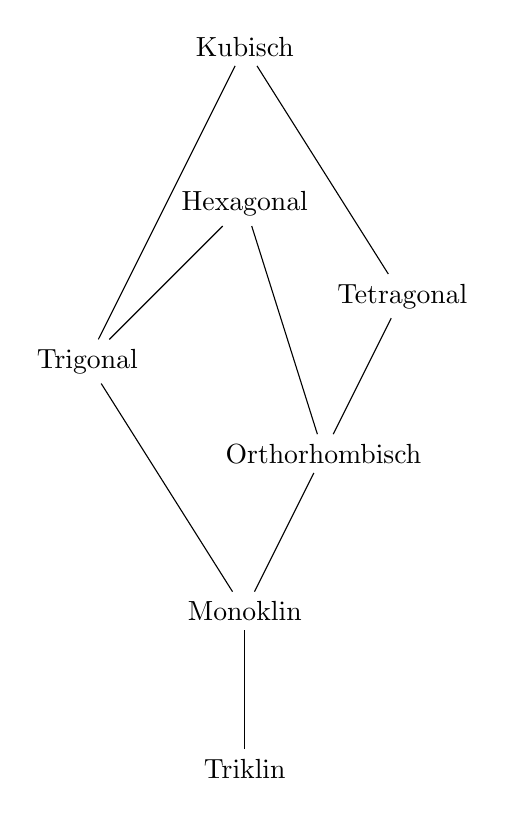
\begin{tikzpicture}[yscale=2]
\node (kubisch) at (0,4.585) % ~\log_2(24) = \log_2(6)+2
	{Kubisch};
\node (hexagonal) at (0,3.585) % ~\log_2(12) = \log_2(6)+1
	{Hexagonal};
\node (tetragonal) at (2,3)
	{Tetragonal};
\node (trigonal) at (-2,2.585) % ~\log_2(6)
	{Trigonal};
\node (orthorhombisch) at (1,2)
	{Orthorhombisch};
\node (monoklin) at (0,1)
	{Monoklin};
\node (triklin) at (0,0)
	{Triklin};

\path
(triklin) edge (monoklin)
(monoklin) edge (orthorhombisch)
(monoklin) edge (trigonal)
(orthorhombisch) edge (hexagonal)
(orthorhombisch) edge (tetragonal)
(tetragonal) edge (kubisch)
(trigonal) edge (kubisch)
(trigonal) edge (hexagonal);
\end{tikzpicture}
\label{kristalle:hasse_diagramm_kristallsysteme}
\caption{Hasse-Diagramm der sieben dreidimensionalen Kristallsysteme}
\end{figure}

\begin{theorem}[Geometrische Einschränkungen]\label{kristalle:kristallographische_einschränkung}
Sei $\Lambda\subseteq\IR^n$ ein Kristall und $1\neq g\in\Aut(\Lambda)$ eine Drehung oder Schraubung um den Winkel $\alpha$.
\begin{enumerate}
\item Die einzigen möglichen Winkel sind $\SI{180}{\degree}=\frac{2\pi}{2}, \SI{120}{\degree}= \frac{2\pi}{3}, \SI{90}{\degree}=\frac{2\pi}{4}$, $\SI{60}{\degree}=\frac{2\pi}{6}$ oder $\alpha=0$.
\item Ist $\alpha\neq 0$, dann gibt es unabhängige Vektoren $v_1, v_2, v_3$ im Translationsgitter (nicht notwendigerweise eine Basis des Translationsgitters), sodass
\begin{enumerate}
\item $v_1$ in Richtung der Drehachse von $g$ zeigt und
\item $v_2$ und $v_3$ senkrecht auf $v_1$ stehen,
\end{enumerate}
Ist außerdem $\alpha\neq\pi$, dann können wir zusätzlich auch
\begin{enumerate}[resume]
\item $v_3={^g v_2}$
\end{enumerate}
erreichen.
\end{enumerate}
\end{theorem}
\begin{proof}
Wir betrachten die orthogonale Abbildung $R_g:=w\mapsto{^g w}$ auf dem Translationsgitter. In unserem Fall ist das eine Drehung.

Die Drehachse geht natürlich durch den Nullpunkt, aber weil wir mit Translationen verknüpfen können, hat das Translationsgitter natürlich auch Drehsymmetrien mit gleichem Winkel und paralleler Drehachse durch jeden anderen Punkt des Gitters.

Wir legen uns das Koordinatensystem so, dass die $z$-Achse in Richtung der Drehachse zeigt und betrachten einen beliebigen Vektor $v=\begin{psmallmatrix}x\\y\\z\end{psmallmatrix}$ im Translationsgitter, der nicht in Richtung der Drehachse zeigt, d.h. $(x,y)\neq(0,0)$. Solche Vektoren gibt es, z.B. müssen immer mindestens zwei Vektoren in jeder Basis des Gitters diese Eigenschaft haben. O.B.d.A. können wir sogar annehmen, dass wir das Koordinatensystem so gewählt haben, dass $y=0$ ist.

\medbreak
Da $R$ das Translationsgitter auf sich selbst abbildet, sind $Rv$ und $R^{-1}v$ wieder Vektoren im Gitter. Wir können explizit beschreiben, was $Rv$ und $R^{-1}v$ sind:
\[Rv =\begin{pmatrix}\cos(\alpha)x\\\sin(\alpha)x\\z\end{pmatrix}, R^{-1}v =\begin{pmatrix}\cos(\alpha)x\\-\sin(\alpha)x\\z\end{pmatrix}\]
Daraus folgt, dass der Gittervektor $v_2:=Rv+R^{-1}v-2v$ die Form
\[(R+R^{-1})v-2v = \begin{pmatrix}(2\cos(\alpha)-2)x\\0\\0\end{pmatrix}\]
hat.

Kann dies der Nullvektor sein? Das geht nur, wenn $2\cos(\alpha)-2=0$, d.h. $\alpha=0$ ist. Ansonsten haben wir einen von Null verschiedenen Vektor $v_2$ im Gitter gefunden, der senkrecht zur Drehachse ist.

Wenn wir noch einen zweiten, Vektor $v'$ nehmen, der von $v$ und der Drehachse linear unabhängig ist (z.B. wieder einen Basisvektor), dann können wir auf dieselbe Weise einen von $v_2$ linear unabhängigen Vektor $v_3$ finden, der senkrecht zur Drehachse ist. Wenn $\alpha$ nicht zufällig $\pi$ ist, dann ist $Rv_2$ auch linear unabhängig von $v_2$ und senkrecht zur Drehachse.

\medbreak
Wir betrachten also zwei Gitterpunkte $A\neq B$ mit Differenzvektor $v_2$, die in einer  Ebene senkrecht zur Drehachse liegen (z.B. den Nullpunkt und $v_2$ selbst). Daraus können wir die Punkte $A'$ und $B'$, indem wir die Drehungen anwenden, deren Achsen durch $A$ bzw. $B$ laufen.

Rechnen:
\[B=A+v_2, \qquad B'=A+Rv_2\]
\[A=B-v_2, \qquad A'=B-R^{-1}v_2\]
Die Punkte $A'$,$B'$ sind selbst Gitterpunkte, d.h. ihre Differenz $B'-A'=(A-B)+Rv_2+R^{-1}v_2=(R+R^{-1}-1)v_2$ ist selbst wieder ein Vektor im Translationsgitter. Wir rechnen nach: Wenn $v_2=\begin{psmallmatrix}x_2\\0\\0\end{psmallmatrix}$ ist, dann ist
\[(R+R^{-1}-1)v_2 = \begin{pmatrix}(2\cos(\alpha)-1)x_2\\0\\0\end{pmatrix}\]
d.h. $(R+R^{-1})v_2-v_2$ ist ein Vielfaches von $v_2$. Da beides Gittervektoren sind, ist das nur möglich, wenn es sich um ein \emph{ganzzahliges} Vielfaches handelt, d.h. $2\cos(\alpha)-1$ muss eine ganze Zahl sein!

Die einzigen möglichen Werte für $\alpha\in[0,\pi]$, die das erfüllen, sind:
\[\begin{array}{c|ccccc}
\alpha & 0 & \frac{2\pi}{6} & \frac{2\pi}{4} & \frac{2\pi}{3} & \pi \\
\hline
\cos(\alpha) & 1 & \frac{1}{2} & 0 & -\frac{1}{2} & -1 \\
2\cos(\alpha)-1 & 1 & 0 & -1 & -2 & -3 \\
2\cos(\alpha)-2 & 0 & -1 & -2 & -3 & -4
\end{array}\]
Das zeigt schon einmal, dass nicht beliebige Winkelwerte für Drehungen eines Translationsgitters vorkommen können.

\medbreak
Kehren wir zurück zu $v=\begin{psmallmatrix}x\\0\\z\end{psmallmatrix}$ und $v_2=\begin{psmallmatrix}(2\cos(\alpha)-2)x\\0\\0\end{psmallmatrix}$. Aus der Tabelle mit den expliziten Werten lesen wir ab, dass für $k\in\set{1,2,3,4}$ der Gittervektor $v_1:=v_2+kv=\begin{psmallmatrix}0\\0\\kz\end{psmallmatrix}$ in Richtung der Drehachse liegt.
\end{proof}

\begin{remark}
Das schließt also insbesondere auch aus, dass es Kristalle mit Dodekaeder-Symmetrien gibt, denn ansonsten müsste es Drehungen der Ordnung 5 im Translationsgitter geben.

Mehr Einschränkungen gibt es jedoch nicht mehr, d.h. jede der endlichen Drehgruppen, die ausschließlich 2-, 3-, 4- oder 6-zählige Symmetrien hat, kommt tatsächlich in der Symmetriegruppe eines dreidimensionalen Kristalls vor.

Der hier vorgestellte Beweis verallgemeinert sich nicht auf höhere Dimensionen. Je höher die Dimension ist, desto höher kann die Ordnung der vorkommenden Drehungen sein. Beispielsweise hat das $n$-dimensionale Würfelgitter $\IZ^n$ eine Symmetrie der Ordnung $n+1$. Insbesondere gibt es im $\IR^4$ schon Kristalle mit 5-zähligen Symmetrien.
\end{remark}

\begin{example}
\begin{enumerate}
\item Der Kristall $\IZ^3\subseteq\IR^3$ hat die Würfelgruppe in seiner Symmetriegruppe. Also besitzt er sowohl 3- als auch 4-zählige Drehsymmetrien. Wenn es eine 4-zählige Drehung gibt, gibt es auch eine 2-zählige.
\item Der Kristall $(\IZ+(\frac{1+\sqrt{3}i}{2})\IZ) \times \IZ \subseteq \IC\times\IR = \IR^3$ (Honigwaben) hat eine 6-zählige Drehsymmetrie.
\end{enumerate}
\end{example}

\begin{remark}
Wenn wir linear unabhängige Vektoren $v_1,v_2,v_3\in Trans(\Lambda)$ gefunden haben, z.B. mit Hilfe der obigen Konstruktion, dann ist $T_0:=\IZ v_1+\IZ v_2+\IZ v_3 \leq Trans(\Lambda)$ ein Untergitter, das ggf. weniger Gittervektoren enthält und eine größere Basiszelle hat. Die so konstruierte Basiszelle ist vielleicht größer als sie sein müsste (sie ist also keine \emph{elementare} Basiszelle), kann aber den Vorteil haben, geometrisch einfacher zu sein als eine elementare Basiszelle, z.B. ist in der Situation des obigen Satzes $v_2$ und $v_3$ senkrecht auf $v_1$. Es muss keine Basis von $Trans(\Lambda)$ geben, die diese Eigenschaft besitzt.
\end{remark}

\begin{proof}[Beweis der Klassifikation der Kristallsysteme]
Es ist $G\leq O(\IR^3)$ und somit $D:=G\cap SO(\IR^3)$ eine Untergruppe von $G$, die Untergruppe aller \emph{orientierungserhaltenden} Symmetrien. Man beachte nun, dass wir stets die Inversion im Nullpunkt in $G$ enthalten haben, da dies immer eine Symmetrie von $T$ ist (es muss keine Symmetrie des $T$ zugrundeliegenden Kristalls sein).

Jedes Element $g\in G$ ist entweder bereits in $D$ enthalten oder $-g$ ist in $D$ enthalten. Daher ist $G=\Set{\pm g | g\in G} = \braket{-1,D}$. Es genügt also, die möglichen Drehgruppen zu klassifizieren. $G$ (und damit auch $D$) ist endlich, weil es eine kristallographische Punktgruppe ist. Wir kennen aufgrund von \ref{gruppen:klassifikation_drehgruppen_in_3D} alle möglichen, endlichen Drehgruppen und aufgrund von \ref{kristalle:kristallographische_einschränkung} können aber nur solche Drehgruppen auftreten, in den alle Drehungen Ordnung 1,2,3,4 oder 6 haben. Das reduziert unsere Liste auf genau die angegebenen Gruppen.
\end{proof}